\section{Track Trigger System Architecture\label{sec:tracktrigger}}


\subsection{CMS Outer Tracker Design and Simulation }


\subsection{System Architecture concept: divide and conquer in space and time }

	Processing each beam crossing implies finding and fitting thousands of tracks starting from a collection of Pt "stubs" (hit pairs, to be described earlier). We need to process 40 million beam crossing per second with a maximum latency of order of a few microseconds. The total raw computation power needed to solve this problem is huge, several orders of magnitude larger than what has ever been used for L1 triggering in the past. We obviously need to resort to massive parallelism and we choose to process in parallel different crossings coming at different times (time multiplexing) and different regions of the detector for the same crossing (regional multiplexing). For this purpose we divide the detector into 48 angular regions (n in $\eta$ times m in $\phi$) we call "towers". We assign multiple processing engines to each tower so that data from that  tower and from different crossings may be processed in parallel. In such a parallel system, a significant  problem we need to address and solve is how to dispatch the right data to the right processors. Data from the same crossing, coming from different detector elements, must be assembled and delivered to the same processing unit for track reconstruction. Data from different crossings, coming from the same detector element, must be delivered to different processing units for optimal time multiplexing. The subdivision of the detector into geographical towers, does not lead to an exact corresponding subdivision of the track parameter space. Data coming from a given geographical tower may need to be delivered to multiple parameter space regions. This happens, in particular, when a stub comes from a detector element close to the border between geographical towers, due to the finite curvature of charged particles in the magnetic field and finite size of the beam luminous region along the beam axis. In addition to the complex data dispatching challenge, there is the obvious challenge of finding and fitting many billions of tracks every second which requires extremely fast pattern recognition algorithms. 

 Current estimates show that only four microseconds will be available for track finding and fitting at L1. This includes data dispatching for trigger tower formation, pattern recognition, track fitting.  Data dispatching is where the stubs from many thousands silicon modules must be organized and delivered to the appropriate eta-phi trigger towers. Due to the finite size of the beam's luminous region in z and the finite curvature of charged particles in the magnetic field, some stubs must be duplicated and sent to multiple towers in an intelligent way. Since all this must be done within a very short time (of the order of a micro-second), communication between processing elements in different towers requires very high bandwidth and very low latency. In addition, extremely fast pattern recognition and effective track fitting is also required. Extensive $R\&D$ and experimentation of innovative ideas is obviously needed in these areas, and much of what have been done will be described in this paper.

	For the reasons above, the design of the overall architecture is focused on the need for efficient dispatching of the data for time and regional multiplexing and on the capability of providing a common flexible framework to test different possible solutions for track finding and fitting. Since the efficient data dispatching for time and regional multiplexing requires high bandwidth, low latency, and flexible real time communication among processing nodes, a full mesh communication based architecture is a natural fit. The full-mesh communication architecture can be implemented either with optical fibers or backplane. A custom ATCA board called Pulsar II, using the ATCA full-mesh backplane,  has been developed at Fermilab with the goal of creating a scalable architecture abundant in flexible, non-blocking, high bandwidth board-to-board communication channels. The Pulsar II hardware is the workhorse for the vertical slice demonstration. In addition, a pattern recognition mezzanine card is developed, as the pattern recognition engine. The full-mesh ATCA backplane permits high bandwidth inter-board communication. The full-mesh backplane is used to time-multiplex the high volume of incoming data in such a way that I/O demands are manageable at the board and chip level. The resulting architecture is scalable, flexible and enables us to provide an early technical demonstration using existing technology. The ATCA architecture allows us to explore and compare various pattern recognition architectures and algorithms within the same hardware platform. The detals of the Pulsar II hardware will be escribed later.
	
\noindent Track reconstruction typically consists of two steps: pattern recognition followed by track fitting. Pattern recognition involves choosing, among all the hits present in the detector, those hits that were potentially caused by the same particle. This stage produces a set of ”hits of interest”. Track fitting involves extracting track parameters from the coordinates of the ”hits of interest”. When time constraints are not so stringent, track reconstruction is implemented in software, often using processors running in the upper levels of a data acquisition system. However, software algorithms running on standard CPUs are typically not fast enough for low level triggers. 
 Hardware-based pattern recognition for fast silicon-based triggering on charged tracks was first developed for the CDF Silicon Vertex Trigger (SVT) at the Fermilab Tevatron in the 1990's.  The method used there~\cite{bib:Rist-89} was based on a massively parallel architecture - the Associative Memory - to efficiently identify patterns at high speed, and has provided an effective solution to fast track triggers in a hadron collider environment. It was successfully used in CDF in Run II at trigger Level 2 enabling a large number of physics results over more that 10 years. The same approach is now being implemented for ATLAS (FTK), also at Level 2, albeit with a much improved hardware architecture implemented with modern technology. However, applying associative memory approach to CMS Level 1 tracking trigger will require extensive $R\&D$ at all stages. 


	


\subsubsection{Tracker geometry and Trigger Towers }

\noindent Many unique challenges must be faced at the different stages of the processing chain: first, data need to be transferred out of the tracker at the necessary speed, stubs from thousands of silicon modules must be formatted, organized into $\eta - \phi$ trigger towers, duplicated and shared across tower boundaries as needed, then we need to perform pattern recognition and track fitting, and finally process all the tracks reconstructed by the previous stages to form an intelligent trigger decision. A coherent system design for a Level-1 track trigger will include all these aspects.

\noindent For the purpose of demonstration, we will make the working assumption that there will be a total of about 15K detector modules/fibers, each fiber with 5-10~Gbps payload bandwidth capability. The detector will be partitioned into 48 trigger towers, 6 in $\eta$ and 8 in $\phi$. Each trigger tower will therefore handle ~300 modules/fibers on average. The cabling of the modules will need to be optimized for trigger requirements. For simplicity, we will assume that the DAQ system are upstream and receive the fibers from the modules and pass the relevant data to the track trigger system. The focus here is the Vertical Slice Demonstration System, not the DAQ readout, so the DAQ readout details do not have to be involved in the demonstration.


\noindent The found stubs are sent from the modules using a block synchronous data transfer scheme which tolerates random occupancy fluctuations while bonding latency. The current plan is to have the data from 8 consecutive beam crossings as one block. The front-end designers are still investigating different format variants for robustness against rate fluctuations, ease of implementation, impact on power consumption, etc. While choosing the 8 crossings scheme as our current working assumption, our strategy is to design the downstream components to be flexible enough to handle different possible formats. 

\noindent Detailed studies have been done for the Barrel-Endcap (BE) tracker geometry with different trigger tower partitions, and the 6 (in $\eta$) x 8 (in $\phi$) = 48 trigger tower partition has been chosen as the default baseline configuration (see Figures~\ref{fig:SecDef_RZ}).

\begin{figure}[ht!]
\centering
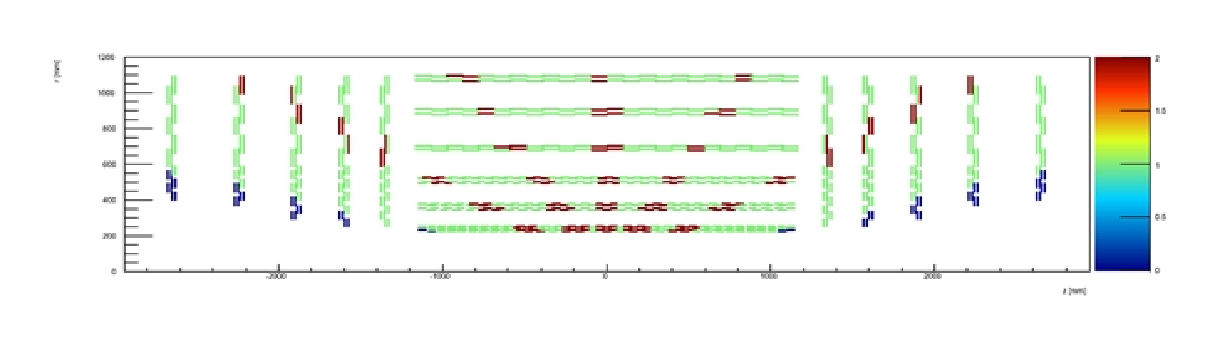
\includegraphics[width=0.75\columnwidth]{Plots/SecDef_RZ.eps}
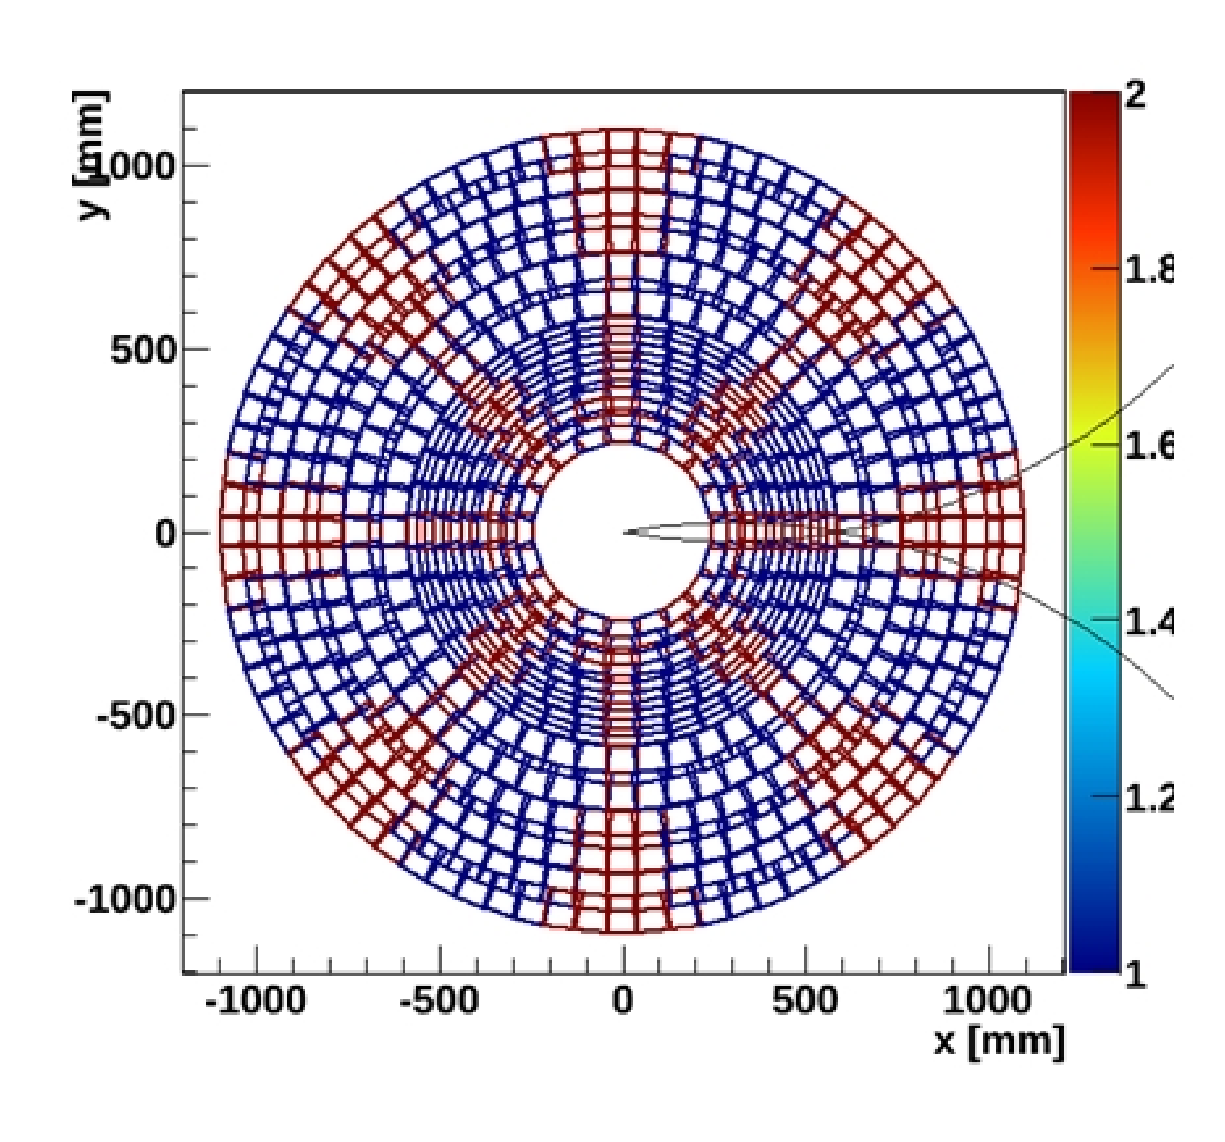
\includegraphics[width=0.2\columnwidth]{Plots/SecDef_XY.eps}
\caption{Six sectors in $\eta$ (left). Note that the symmetry around $\eta=0$ will provide for easier cable grouping. Eight sectors in phi (right).}
\label{fig:SecDef_RZ}
\end{figure}


\noindent Stubs from the 15K silicon modules must be delivered to the correct trigger towers. 
%Due to the finite size of the beam's luminous region in z and the finite $p_T$ curvature of charged particles in the magnetic field, some of %the stubs, coming from the neighborhood of some tower boundary, must be delivered to multiple towers to avoid efficiency gaps.  
Detailed studies have been performed on data sharing assuming the default 48 tower partition with a minimum $p_T$ of 2 GeV and track origin smearing in $z\pm 7$ cm. Figure~\ref{fig:TT_config} shows the number of trigger towers that stubs from a given module must be delivered to under these conditions. When a stub is in the middle of the trigger tower, it will have to be delivered to only one tower (to the native trigger tower). When a stub is at the boundary in phi or eta (but not both), it will have to be delivered to two towers. If a stub is at both the boundaries in eta and phi, it will have to be delivered to four towers. Note that four towers is the maximum number of towers any stub must be delivered to. 



\noindent The subdivision of the tracker into 48 trigger towers is shown in Figure~\ref{fig:TT_config} (right), where the colored lines indicate all needed interconnections among the trigger towers. The unique feature of this arrangement is that any given trigger tower only needs to be connected and share stubs with its immediate eight neighbors and detailed studies show that this feature is more or less independent from the minimum $p_T$ threshold and track origin smearing in $z$ requirements. This inter-connection structure will be used as the basis of the proposed trigger system architecture. 

\begin{figure}[ht!]
\centering
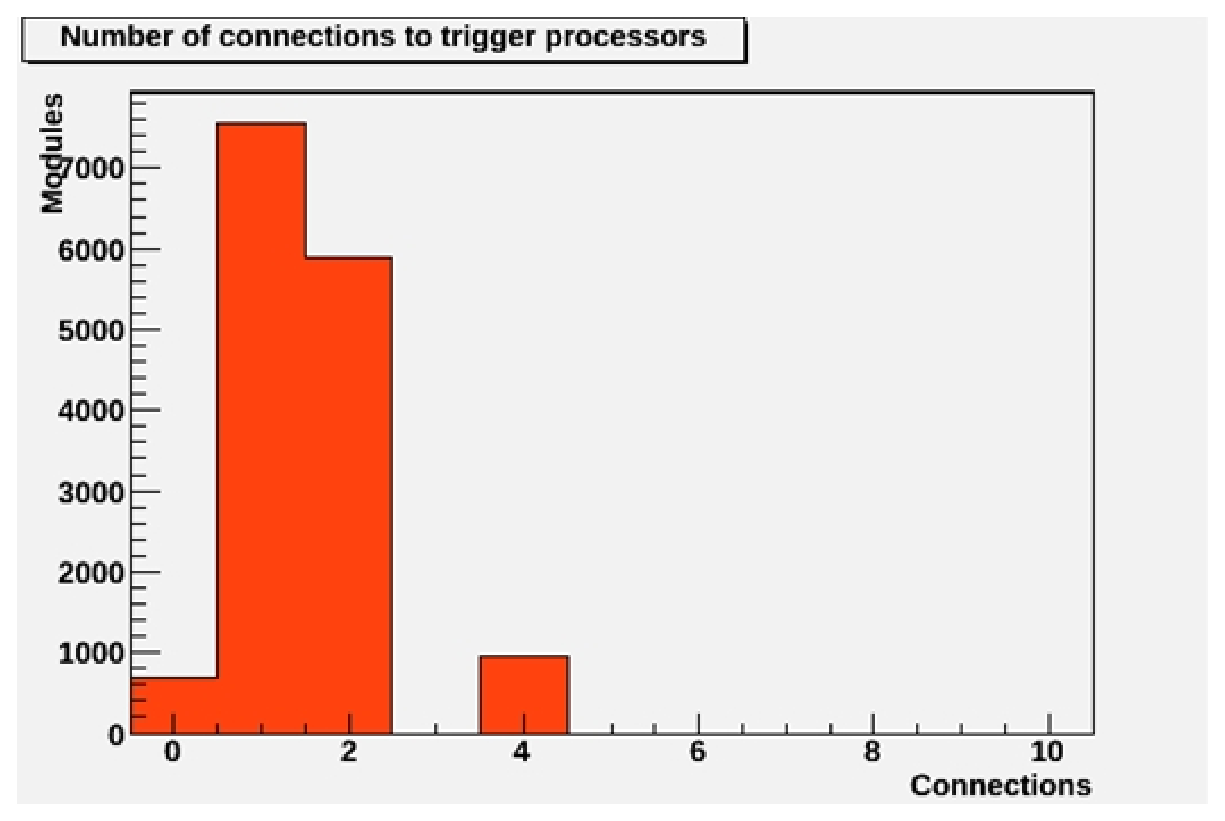
\includegraphics[width=0.45\columnwidth]{Plots/SecDef_N.eps}
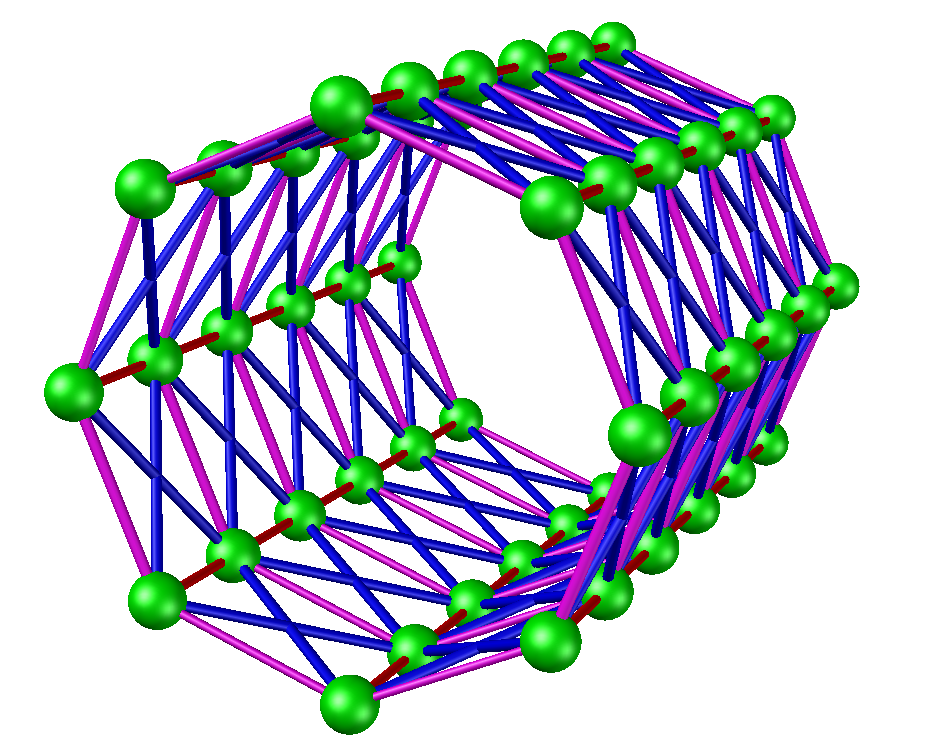
\includegraphics[width=0.5\columnwidth]{Plots/CMS_L1_48_towers.png}
\caption{
Left: Distribution of the number of trigger towers each module needs to be connected to. Entries at zero are from modules that do not participate in triggering.
Right: Conceptual view of the proposed CMS phase II L1 tracking trigger towers.  The formation is organized as 48 trigger towers (6 $\eta$ x 8 $\phi$).  Because the phase II tracker is being designed for tracking trigger purposes, it is possible to arrange the towers in such a way that data sharing only requires communication with immediate neighbor towers.  Each node in this diagram represents a trigger tower processor engine.  Within each processor engine crate the full mesh backplane is used for time multiplexing of the incoming data, while the data sharing between towers is handled with inter-crate fiber links.}
\label{fig:TT_config}
\end{figure}



\subsubsection{System Architecture}

\noindent The tower processor platform must support large numbers of fiber transceivers, which are used for receiving input links and sharing data between neighboring towers.  A flexible, high bandwidth backplane is also required to quickly transfer data between boards.  The boards should be large enough to support pattern recognition engines and fiber connections. Given these requirements, we conclude that a full mesh 14 slot ATCA shelf is a natural fit for the tower processor. An ATCA shelf is typically an air-cooled 13U rack mounted chassis consisting of 14 slots.  The first two slots are reserved for Ethernet switch blades.  Switch blades may include a fast CPU and are often used for controls and other system functions.  The remaining 12 slots are used for processor or payload blades.  In a full mesh ATCA backplane each pair of slots is directly connected with a multi-lane bidirectional serial channel capable of supporting sustained 40+ Gbps data transfers.  A modern "40G+" full mesh ATCA shelf has a total aggregate bandwidth of over 7 Tbps, not including external I/O. As mentioned earlier, the full-mesh communication concept can be implemented either using full-mesh backplane, or using optical fibers. For  demonstration purpose, we will use the full-mesh backplane here. 

\noindent For simplicity and illustration purpose, let's simply assume one ATCA shelf per trigger tower for the moment as a starting point. This will be the assumption for the vertical slice demonstration. Following this assumption, if we were building the L1 Tracking Trigger system today using existing technology, we could propose a system comprised of 48 ATCA shevles with possibly an additional shelf acting as a second stage processor, as shown in Figs.~\ref{fig:System_1} and~\ref{fig:System_2} . Of course, the actual system will most likely be smaller (e.g. 24 or 12 shelves). Note that connections between tower processor shelves are limited to eight nearest neighbors, and this can be easily achieved.

\begin{figure}[ht!]
\centering
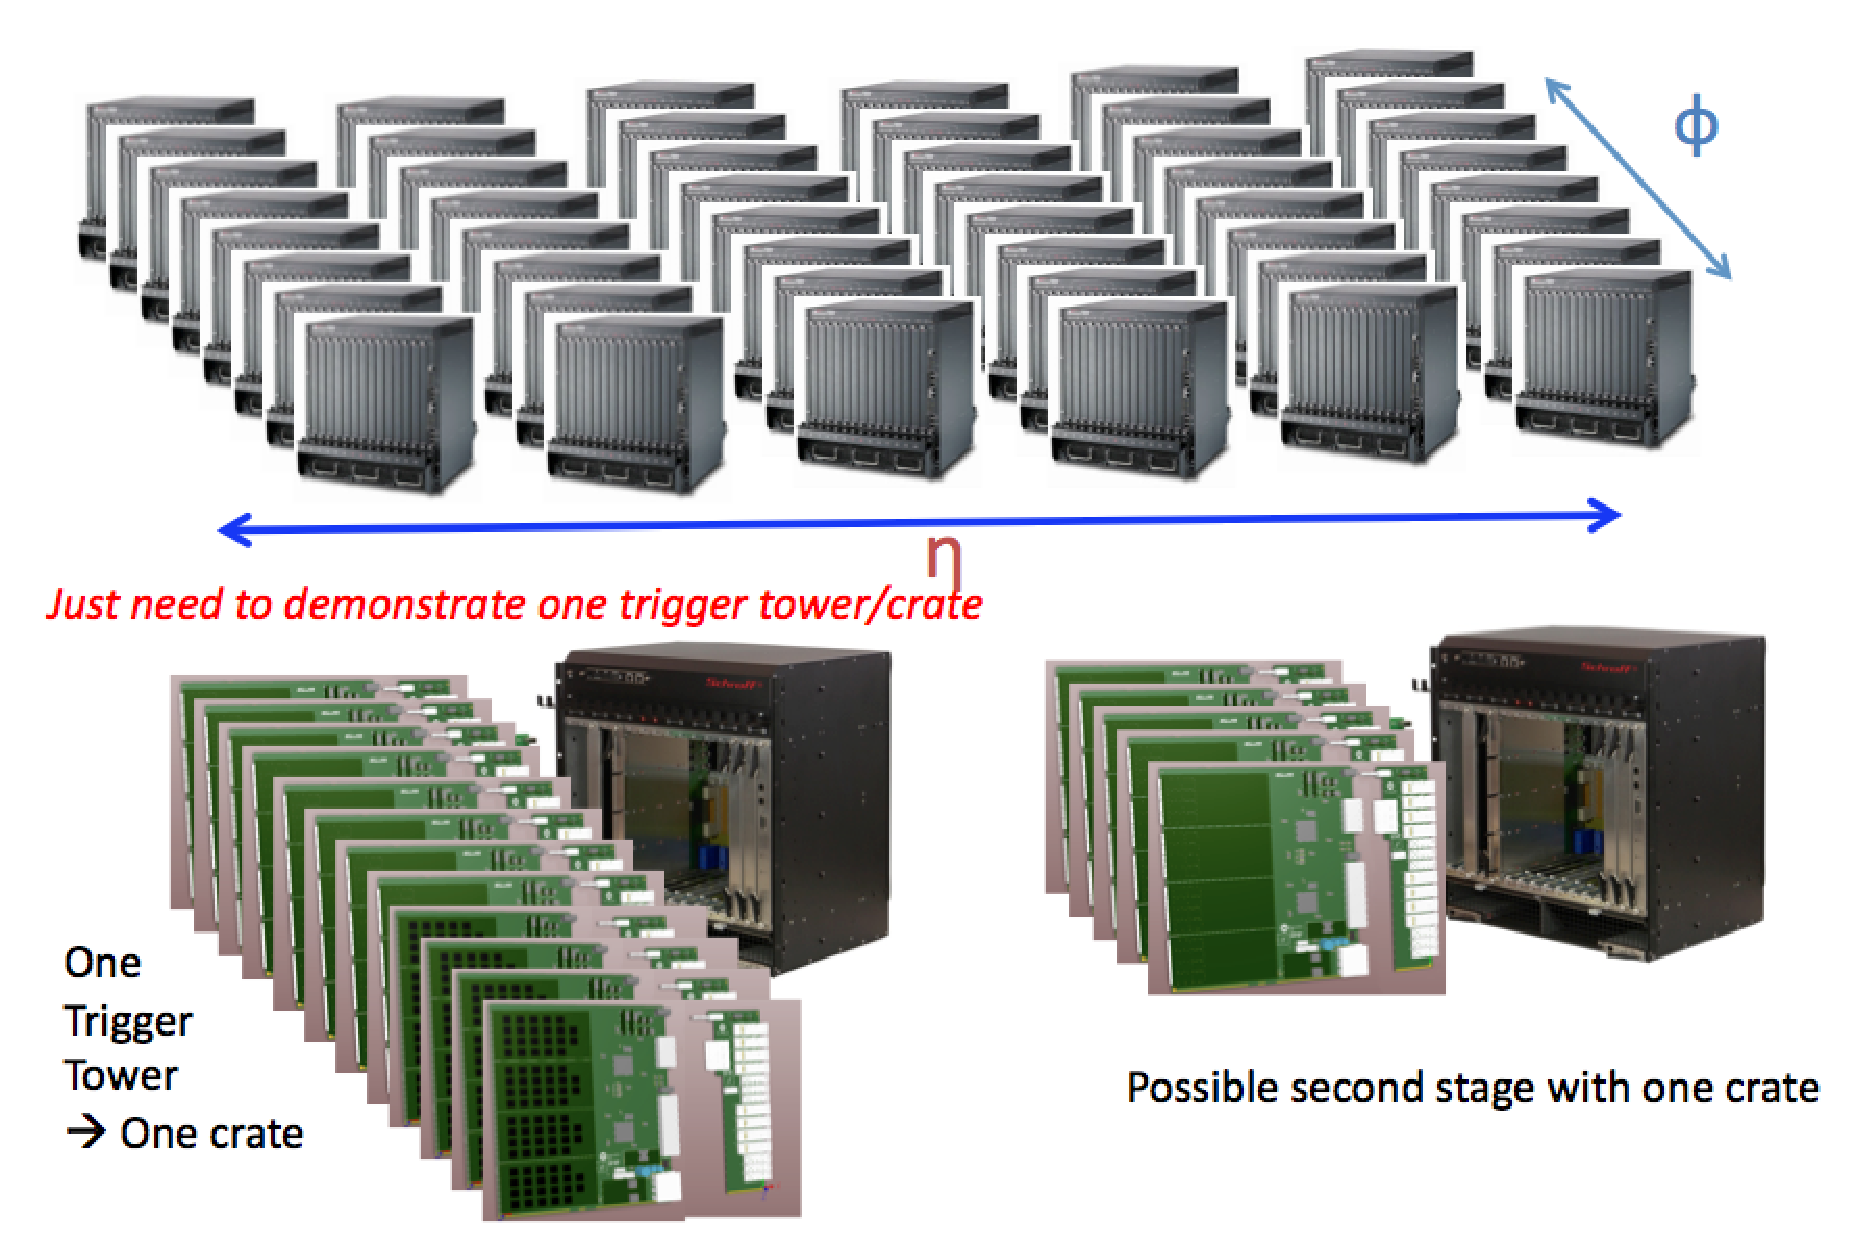
\includegraphics[width=0.7\columnwidth]{Plots/System_1.eps}
\caption{Possible system configuration with today's technology by simply assuming one ATCA shelf per trigger tower (will be smaller in the future for the actual system)}
\label{fig:System_1}
\end{figure}

\begin{figure}[ht!]
\centering
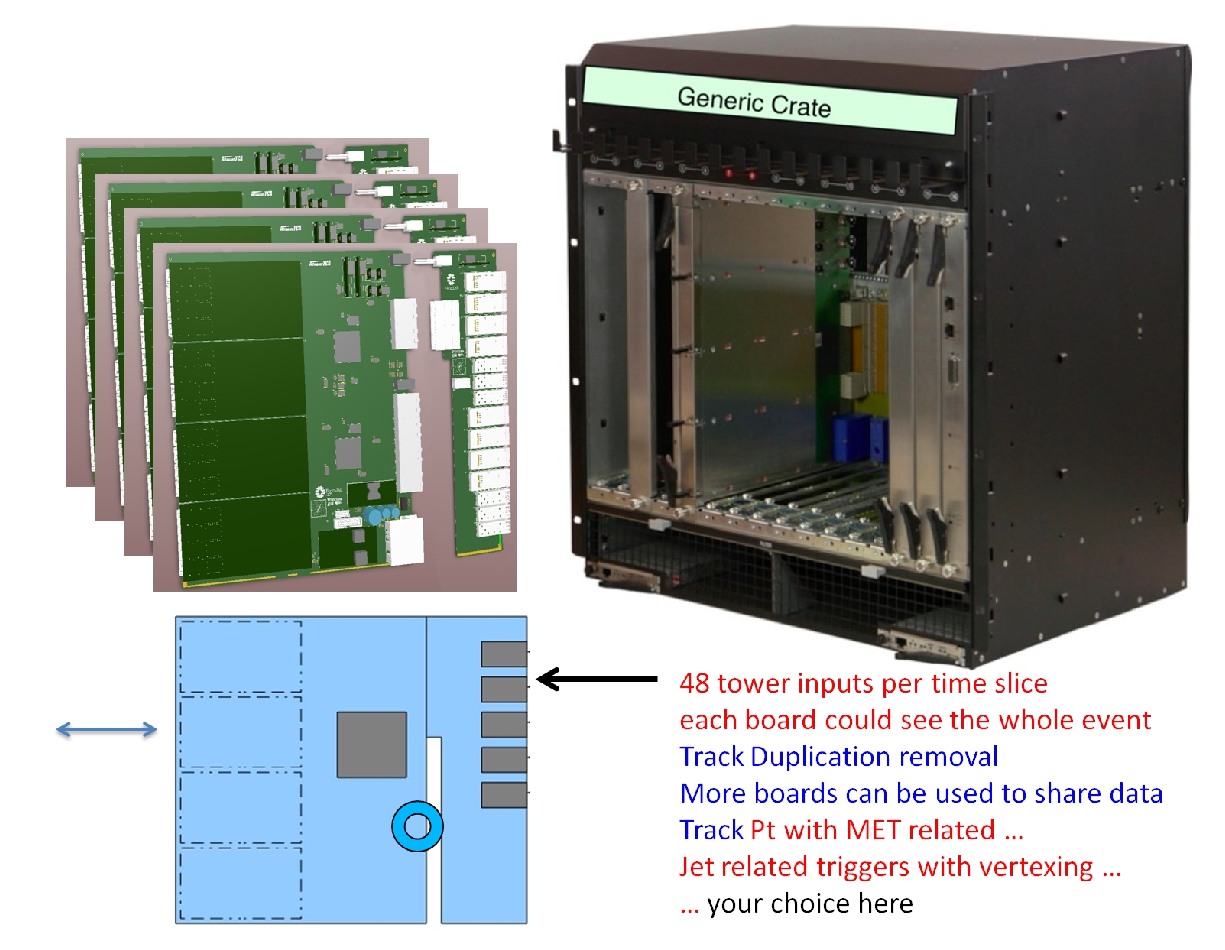
\includegraphics[width=0.5\columnwidth]{Plots/System_2.eps}
\caption{The second processing stage shelf.}
\label{fig:System_2}
\end{figure}



\begin{figure}[ht!]
\centering
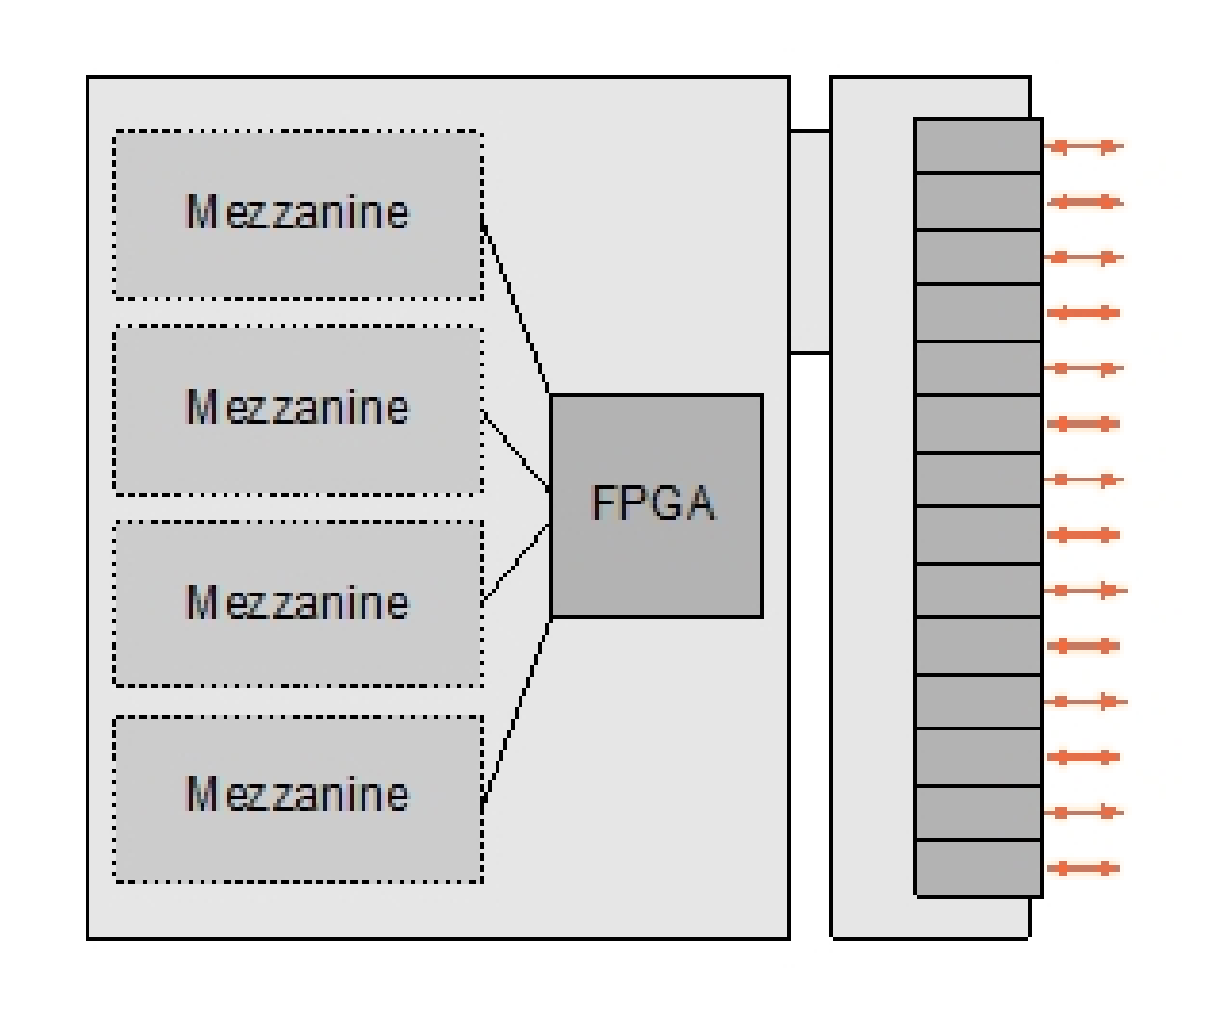
\includegraphics[width=0.4\columnwidth]{Plots/ProcBlade.eps}
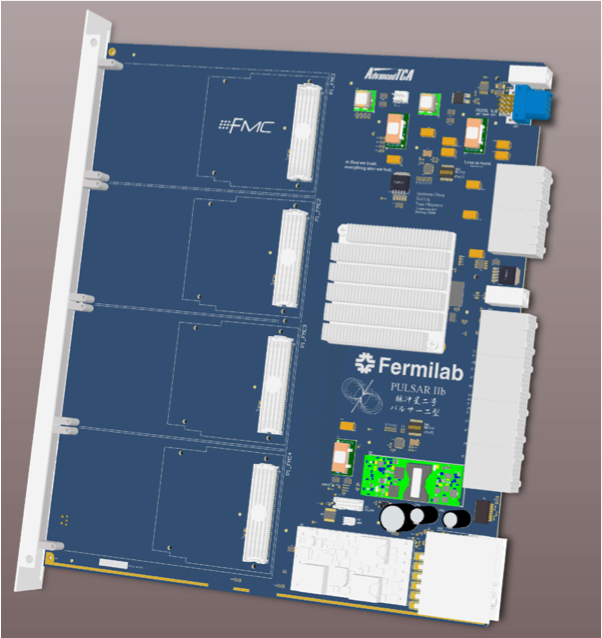
\includegraphics[width=0.4\columnwidth]{Plots/PulsarIIb.png}
\caption{Generic processor blade concept (left), and the actual design of Pulsar IIb~\cite{bib:PulsarII} at final layout stage (right)}
\label{fig:ProcBlade}
\end{figure}

\begin{figure}[ht!]
\centering
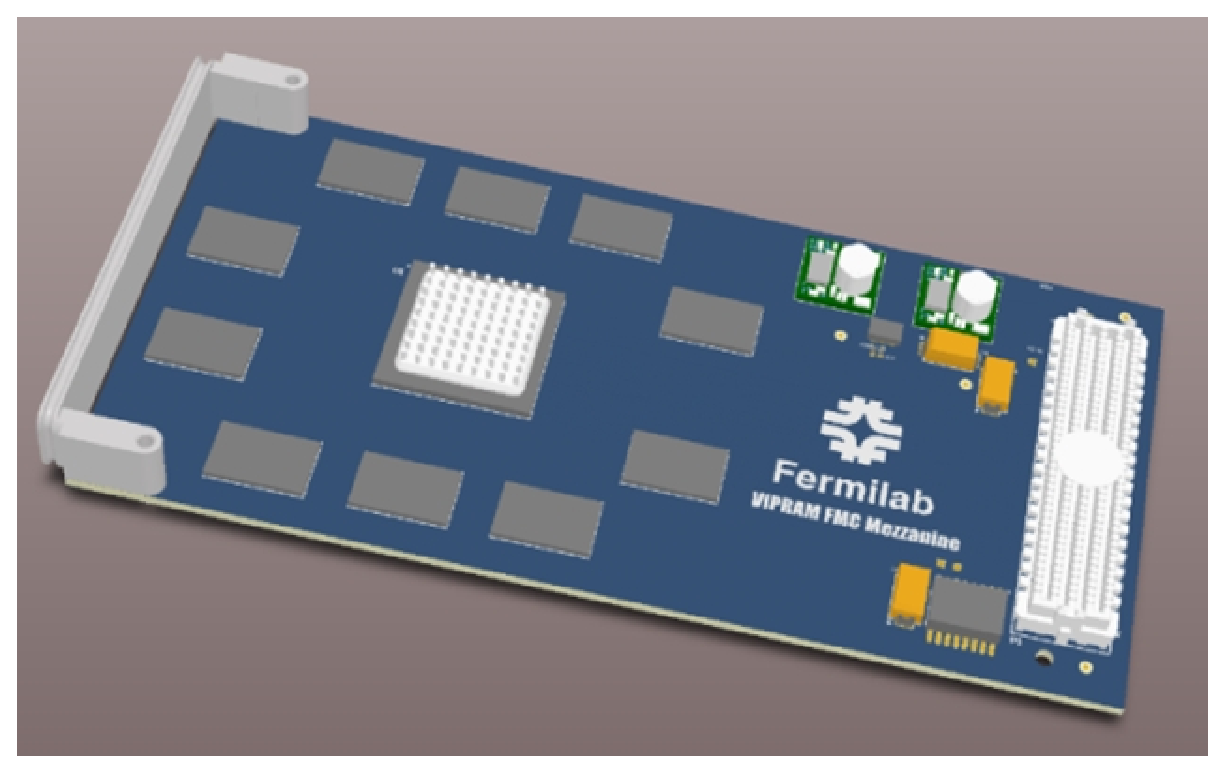
\includegraphics[width=0.4\columnwidth]{Plots/PRAM.eps}
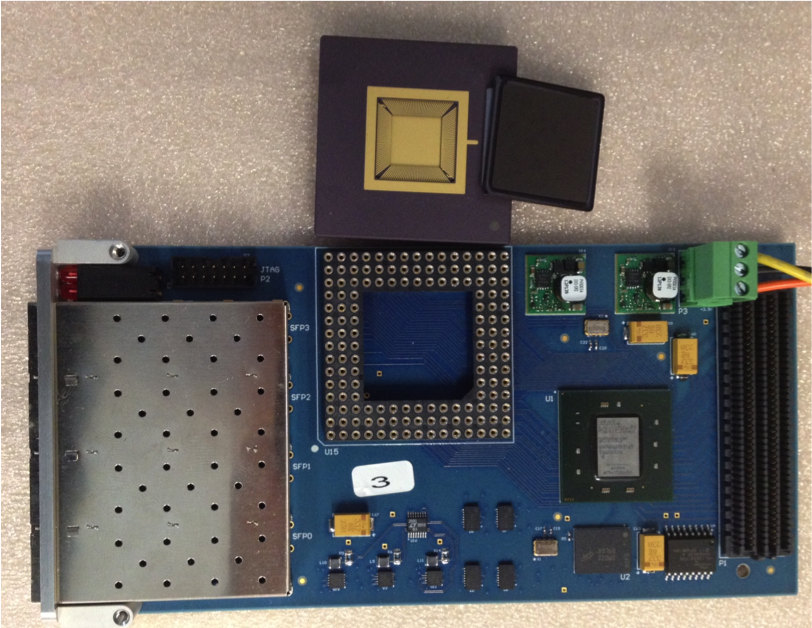
\includegraphics[width=0.4\columnwidth]{Plots/test_mezzanine.png}
\caption{Left: Concept of a pattern recognition mezzanine design for testing different pattern recognition algorithms.
Right: a test mezzanine prototype designed and built at Fermilab, features four SFP+ pluggable serial transceivers (for standalone
data receiving), a Kintex 7 FPGA, configuration flash memory, DDR3 memory, power supplies, local oscillators, a test socket for
associative memory chips developed at Fermilab, and FMC connectors. 
}
\label{fig:PRAM}
\end{figure}

\noindent The generic processor blade concept is shown in Figure~\ref{fig:ProcBlade} (left).  The front board measures 8U x 280mm and is designed around a single FPGA.  This FPGA connects directly to the full mesh backplane fabric, mezzanine cards, and fiber transceivers located on a rear transition module (RTM).  For the most part communication channels are high speed serial point to point links and are directly supported by SERDES transceivers in the FPGA. The actual design of Pulsar IIb is also shown in Figure~\ref{fig:ProcBlade} (right).

\noindent The fundamental processing element is a pattern recognition mezzanine (PRM) card shown on Fig.~\ref{fig:PRAM} which performs both track finding and fitting. Time multiplexed data transfers into several parallel PRMs can reduce bandwidth requirement to manageable level.  PRM's using different approaches to track finding and fitting may be tested and compared within the same overall high-level system architecture and data dispatching scheme.


The system architecture described above is scalable, flexible and, although not meant to be what we
will actually implement in the final system, will enable us to provide an early technical demonstration
of the feasibility of a L1 tracking trigger for CMS. For example, a major advantage of the full mesh
communication (either via optical connection or via backplane) is that it effectively blurs the distinction between boards, thus enabling system architects to
experiment with different shelf configurations. In the following sections we briefly illustrate two kinds of
tower processor systems made possible by the flexibility of the full mesh architecture. (why this paragraph is repeating itself after compilation?....)


The system architecture described above is scalable, flexible.... testing testing.



\noindent

The system architecture described above is scalable, flexible and, although not meant to be what we will actually implement in the final system, will enable us to provide an early technical demonstration of the feasibility of a L1 tracking trigger for CMS. For example,
a major advantage of the full mesh backplane is that it effectively blurs the distinction between boards, thus enabling system architects to experiment with different shelf configurations.  In the following sections we briefly illustrate two kinds of tower processor systems made possible by the flexibility of the full mesh architecture.

\paragraph{N DIB and M PRM configuration ($N+M \le 12$)}

\noindent The most straightforward tower processor architecture consists of N data input boards (DIB), which receive input links and perform zero suppression.  After zero suppression, the N DIBs transfer the event data to M number of pattern recognition boards (PRB), which contain Mx4 pattern recognition mezzanine (PRM) cards.  Data transfers from the DIBs to the PRMs are time multiplexed, thereby the bandwidth requirements can be significantly relaxed.  

\noindent Data entering the PRB can be time multiplexed again and transferred to the four PRMs to further reduce bandwidth requirements and allow for longer processing times.  The full mesh backplane fabric supports any variant of these configurations (assuming that $N+M \le 12$), and different variants may have different demands on hardware. Example variations are sketched on Fig.\ref{fig:System_3} and bandwidth requirements for the worst case scenario (assuming 500 stubs per event per trigger tower) are summarized in Table~\ref{tab:shelves}. Note that current study show that on average, we expect only about 100 to 200 stubs per trigger tower per beam crossing, here we assumed 500 stubs to be conservative. 

\begin{figure}[ht!]
\centering
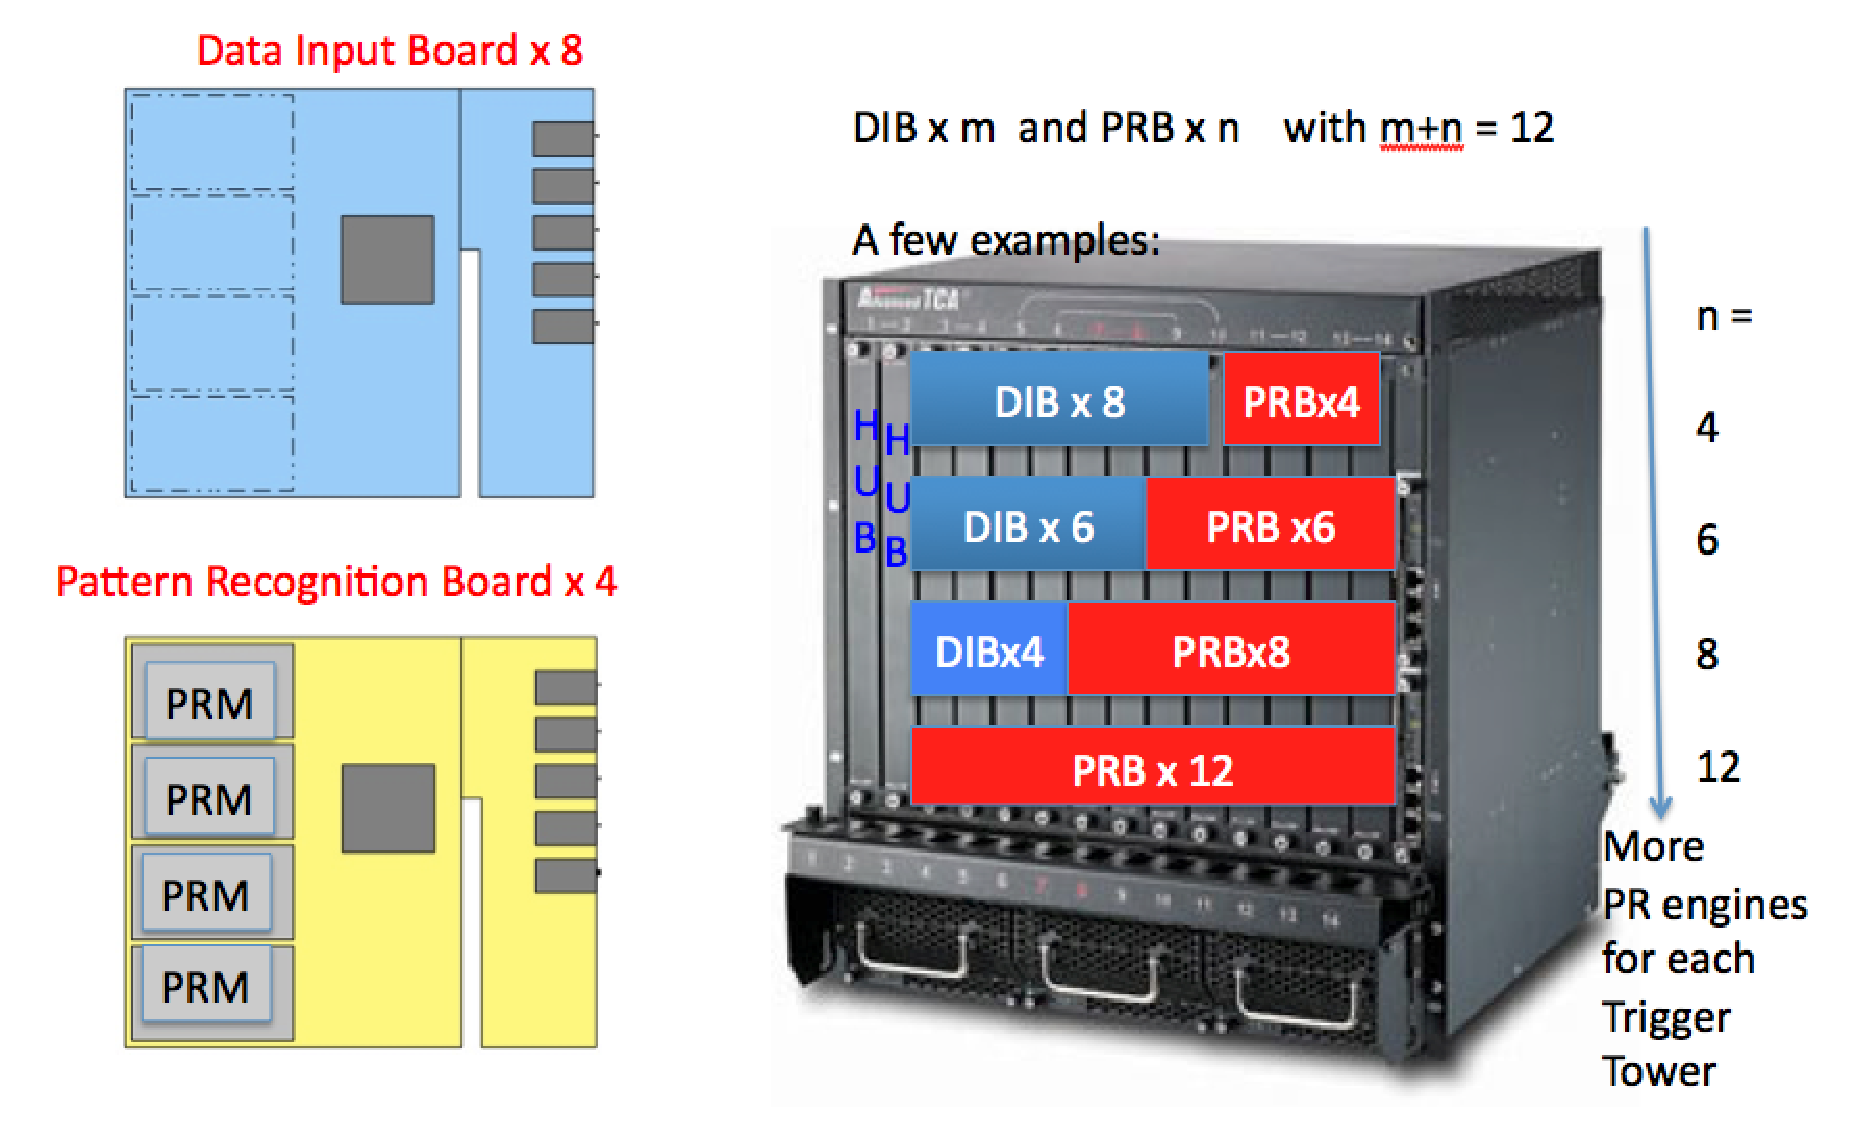
\includegraphics[width=0.7\columnwidth]{Plots/System_3.eps}
\caption{System flexibility: many configurations possible \& being studied to select the right one for demonstration purpose}
\label{fig:System_3}
\end{figure}


\begin{table}[ht!]
\centering\begin{tabular}{|c|c|c|c|c|}
\hline
DIB/PRB/PRM Count &  Fabric Channel BW (minimum)  &	PRM Input BW (minimum) \\
8/4/16 &	20 Gbps &	40 Gbps \\
6/6/24 &	20 Gbps &	27 Gbps \\
4/8/32 &	20 Gbps &	20 Gbps \\
\hline
\end{tabular}
\caption{Data sharing between towers occurs on the PRB board level.  Each PRB connects to the corresponding PRB in the eight nearest tower processor shelves.  The above numbers assume a worst case scenario of 500 32-bit stubs per trigger tower per event (every 25 ns).  An example of special configuration with eight DIBs and four PRBs will be used as a simple example in Section 3.}
\label{tab:shelves}
\end{table}


\paragraph{DIB/PRB combo configuration}

\noindent In the limit of N=0 and M=12 from the "N DIB and M PRB" configuration, the DIB and PRB functionalities can be combined into one blade design.

%\begin{figure}[ht!]
%\centering
%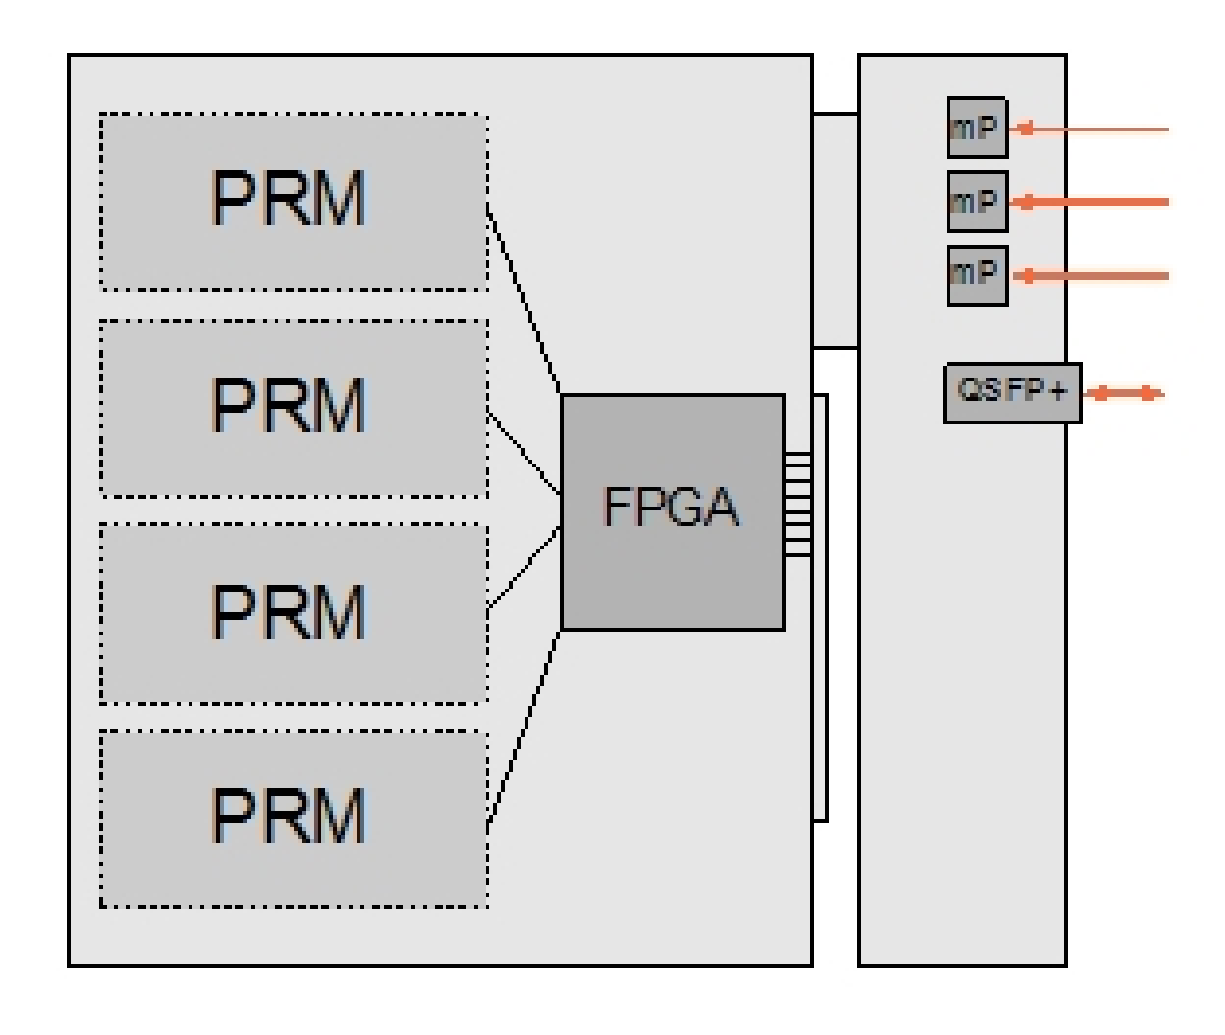
\includegraphics[width=0.45\columnwidth]{Plots/CombBlade.eps}
%\caption{Combined blade design}
%\label{fig:CombBlade}
%\end{figure}


\noindent A tower shelf would then consist of 10 Processor blades, one Gateway blade (for data sharing), and one Collector blade (for tracks found). These three different blade functionalities can be implemented in the same hardware. Backplane transfers are described in a series of fully pipelined sequences shown in Figure~\ref{fig:BackPlaneTr}.

\begin{figure}[ht!]
\centering
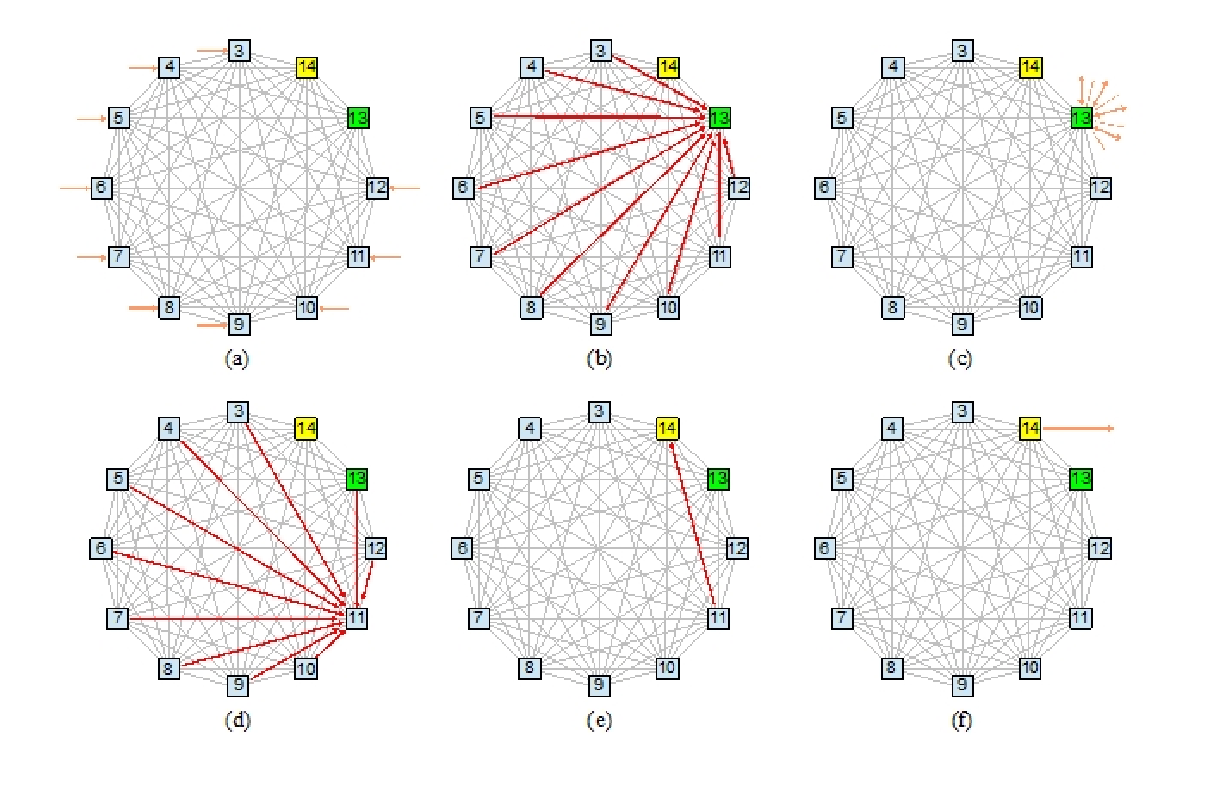
\includegraphics[width=0.9\columnwidth]{Plots/BackPlaneTr.eps}
\caption{Backplane transfers sequences using the combined blade design. First, the input fibers are received on the Processor blades (a).  Each Processor blade then transfers a portion of the input data to the Gateway blade (b), where it is exchanged with neighboring towers over fiber links (c).  The Processor blades and Gateway blade transfer the event (including neighbor data) to the target Processor blade in a time multiplexed, round robin scheme (d).   Results from the Processor blades are then transferred to the Collector blade (e) for any final formatting and processing before transmission downstream (f).}
\label{fig:BackPlaneTr}
\end{figure}
 

\noindent This processor architecture uses every channel in the full mesh backplane.  By using the full mesh fabric more effectively we are able to decrease the channel bandwidth requirement from 20 Gbps down to 6 Gbps with no significant latency increase. 



\section{Applying Associative Memory approach to CMS }




\subsection{Pattern Bank definition and optimization}

\subsection{Definition of superstrips}

	The principle of operation of the Associative Memory requires the surface of the detector to be subdivided into a finite number of elements that we call "superstrips".
	The subdivision into superstrips can be one-dimensional (strips) or bi-dimensional (pixels).
	Any combination of superstrips from different detector layers, compatible with the trajectory of a single valid track, constitutes a valid "pattern". The ensemble of all valid patterns constitutes the "pattern bank" to be loaded into the Associative Memory.
	Deciding the size and shape of the superstrips is the first, and probably the most important, design choice one needs to make in the process of searching for a solution to a specific pattern recognition problem using the Associative Memory approach.
	
	It is immediately intuitive that the superstrips cannot be too large or too small. If the superstrips are made smaller and smaller, then the number of patterns that are needed will grow with a high power of the inverse of the superstrip size and will soon exceed the maximum capacity of the Associative Memory that may be available. On the other hand, if the superstrips are made exceedingly large, then the probability of having multiple hits in the same superstrip will grow and more computing will be required to solve the ambiguities and identify the hits actually belonging to a valid track.
	The amount of information carried by the set of patterns identified by the Associative Memory for a given event, diminishes as the size of the superstrips grows, obviously being reduced to zero in the extreme case when each detector layer is reduced to a single superstrip and, consequently, the pattern bank contains a single pattern.
	Ideally the superstrips should be small enough to ensure that, in most cases, each one will not contain more than a single hit. Here we see how the optimal superstrip size may depend strongly on the occupancy of the detector and how a larger Associative Memory may be required to cope with higher occupancy.
	
	There is also a limit to how small you can sensibly make the superstrips that is connected to the precision of the coordinate measurement. It is quite intuitive that it is of very little value having superstrips much smaller than the measurement error. In fact that would lead to a very large increase in the number of patterns with very small improvement of the information carried by each pattern identified by the Associtive Memory.

	From all this we can understand how the determination of the optimal superstrip size may turn out to be a complex multi-dimensional optimization problem that involves many parameters, including the nature and geometry of the detector, the precision of the coordinate measurement, the characteristics of the tracks we need to identify, the occupancy, the maximum capacity of the Associative Memory that is available and the amount of computing power that is available to solve the residual ambiguities remaining after the Associative Memory has done its job.

	Typical figures of merit to be considered in the optimization of a trigger application may include the total time needed to complete the track finding process (latency), efficiency, rate of fake tracks (purity), precision of track parameter determination.
In the following sections we will describe in some detail the process we followed to optimize the dimension and shape of the superstrips and to generate the pattern bank for the particular problem of the Level 1 tracking trigger for the CMS tracker for the HL-LHC Phase II upgrade.



\subsection{Determination of superstrip size}


We started with the determination of the minimum superstrip size compatible with coordinate measurement errors. The main contribution to measurement error is multiple scattering which  tends to increase as we go from the inner to the outer detector layers because of the increasing amount of traversed material. For this reason we expect the minimum superstrip size to be both layer and momentum dependent.

We used a detailed simulation of the detector to generate a large number of tracks and compare the position of the hits thus produced in each layer with the corresponding ideal position, that is where the hit would be if there were no measurement errors or secondary interactions like multiple scattering. 
The distribution of the simulated tracks in eta and Pt was chosen to resemble as closely as possible what we expect for the HL-LHC run. The minimum Pt value was set at 3 GeV/c.
The difference between the actual and the ideal position along the phi direction was histogrammed for each detector layer independently and the results are shown in Fig.xxx.
Each histogram was integrated, symmetrically starting from the center, to include 90\% of the area and the resulting interval was taken as the size of the superstrips along the phi direction for that layer. The resulting superstrip widths are shown in Table XXX. It can be noted that, due to the increasing amount of material, the size of the superstrips is increasing from the center out even when expressed as angles. It is because of this feature that we named this particular superstrip configuration as "fountain".

During the optimization process, the "fountain" configuration was always assumed as the basis for the superstrip subdivision in the phi direction. When looking for an optimal working point we typically applied a "scale factor" to the "fountain" configuration to vary the size of all the superstrips while maintaining a constant ratio between different layers. When two-dimensional superstrips where used, an orthogonal subdivision in the z direction was added. 



\subsection{Generation of the pattern bank}

To generate a pattern bank we also need to define a "target parameter region". That is the region in track parameter space where we want the maximize the efficiency of the track finding process. That tipically translates to intervals in eta, phi, Pt and coordinates of the origin of the track.

Once the superstrips and the target parameter region are specified, the procedure to generate the pattern bank is, in principle, straightforward. All you need to do is to create a sufficiently large set of simulated tracks within the target parameter region and, for each one of them, record which superstrip it goes through in each detector layer. A pattern is defined as the set of superstrip identifiers (typically integer numbers), one per detector layer. The ensemble of all the different patterns generated by all the tracks in the sample constitutes the "pattern bank".

The "coverage" of a pattern bank is defined as the probability that, given a track randomly extracted within the target parameter region, the pattern it generates is actually present in the pattern bank. In practice it is never possible to reach 100\% coverage, but you typically get closer and closer as you generate more and more tracks and keep adding less and less probable patterns to the pattern bank.
Fig. xxx shows a typical plot of the pattern bank coverage as a function of the size of the pattern bank. You can see how the curve tends to saturate as we are adding patterns that are less and less probable.

During the pattern bank generation process, the same patterns are being hit multiple times and, although we add a particular pattern to the bank only once, we record the number of times it has been hit. This number provides an estimate of the probability of that particular pattern to be hit by a track randomly extracted within the target parameter region. We refer to this probability as "popularity".
A strategy that we have often been using is to start by generating a very large pattern bank, larger than we can reasonably afford given the maximum size of the associative memory we expect to be available. We then sort the patters by decreasing popularity and include patterns in the bank, starting from the most popular, up to the desired coverage or up to the size of the available associative memory. Using the most popular patterns first makes optimal use of the associative memory space.

\subsection{Definition of Trigger Towers}

As explained earlier (xxx), we propose to subdivide the whole tracker into 48 trigger towers and perform track finding in parallel in each one of them. Since some tracks can traverse more than one tower, some detector regions will need to be shared between multiple towers and we need to exercise care in order to avoid track duplication caused by the same track being found in multiple towers.
We first define "virtual" trigger towers as a subdivision of the track parameter space into 48 non overlapping regions. The union of all the 48 regions represents the total parameter space where we want track finding efficiency to be optimized. "Physical" trigger towers are constructed by collecting hits from all detector regions that are needed to obtain full efficiency for all the tracks belonging to one particular virtual tower. Since tracks belonging to different virtual towers can traverse the same physical detector region, it follows that, in general, physical towers overlap (while virtual towers never do). This also solves the problem of potential track duplication because each tower will only accept tracks coming from its own virtual tower and discard possible leaks from neighboring regions.

Fig.xxx is a cartoon showing a possible naive way of defining virtual towers. The parameter space we consider is four-dimensional: phi, Pt, eta, z of the origin. We decompose this four-dimensional parameter space into the cartesian product of two orthogonal two-dimensional spaces. The first space is phi versus Pt (we actually use 1/Pt, mainly because of its regularity through infinite Pt) and the second is eta versus z0 (z coordinate of the origin of the track).
The whole parameter space we want to cover is $Pt > 3$ GeV, $|\eta| < 2.4$ and $|z_0| < 15$ cm.
One simple way to divide this parameter space into 48 non-overlapping regions is to define eight equal intervals in phi and six equal intervals in eta. This is shown in Fig.xxx.

There is some flexibility in the exact way we can define the subdivision of track parameter space into virtual towers, so we can ask ourselves if there is an optimal way to do it. One thing we want to try to minimize is the overlap between adjacent towers. Larger overlaps mean more hits to be fanned out to multiple physical towers and, consequently, larger data traffic and more data processing.

Fig.xxx shows a slightly different way of defining 48 virtual towers. The difference is that the separation between regions is not depending on a single parameter but on a combination of both. This "slant" solution has actually been shown to reduce the overlap between physical towers by a significant fraction (???) with respect to the "straight" solution shown in Fig.xxx. The cartoons in Fig.xxx show how the "straigh" and the "slant" virtual towers translate to physical space and how the overlap regions are changed. For our particular application, the slant angle in both projections was optimized to achieve the minimum amount of overlap between physical towers.

The studies described in what follows are focused on a single trigger tower located in a central eta slice ($0 < \eta < 0.8$). Given the symmetry of the detector, the phi position is irrelevant.



\subsection{Optimization}


The main purpose of these studies was to find at least one viable "working point", that is a pattern bank compatible with the maximum size of the associative memory we believe we can comfortably implement and which, at the same time, would provide sufficient track finding power, to make the remaining pattern recognition, to be performed by the following stages of the tracking trigger, solvable within the allotted maximum latency time.

Pattern banks of different sizes and with different superstrip definitions were generated and the performance of each one of them was studied with Monte Carlo events which included a detailed simulation of HL-LHC collisions with different instantaneous luminosities and of the Phase II upgraded central tracker. 

For each simulated HL-LHC collision, all the tracker hits are fed to the AM. The AM recognizes the patterns that may correspond to a valid track because a sufficient number of superstrips contains at least one hit. All these recognized patterns are passed to the "Data Organizer" stage were all the relevant hits are retrived and attached to each pattern to form a "road". These "roads" will then be fed to the track fitting stage where the possible remaining ambiguities will be solved and track parameters will be extracted.

Given a specific pattern bank, the number of roads generated by the AM for each event is a relevant figure of merit because more roads means more work for the track fitting stage and, consequently, larger latencies. 

The number of roads obviously depends also on the properties of the collision, expecially on the occupancy of the detector. For this study we used a Geant simulation of the Phase II upgraded CMS detector and minimum bias collisions at an instantaneous luminosity corresponding to and average number of collisions per beam crossing of 200 (PU 200).

Fig.xxx shows the number of patterns in the bank versus the number of roads generated for each crossing for different possible definitions of the superstrips. Patterns were added to the pattern bank until a coverage of at least 95\% was reached. 

The distribution of the points clearly shows the nature of the compromise between the size of the pattern bank and the number of roads output by the AM, to be processed by the following stages. The larger the pattern bank, the more pattern recognition power we have in the AM, the less amout of work is left to be done for the following stages of the track finding process.

From this plot we chose, as a baseline working point, the sf1\_z4 (?) pattern bank as a good compromise. That corresponds to a scale factor of 1 for the "fountain" configuration in the phi direction, and four approximately equal segments in the z direction in each one of the six tracker layers. This requires a pattern bank of about 1.6 million (?) patterns and will produce about 200 (?) roads per crossing.

The amount of work that remains to be done by the track fitting stage depends on the number of roads, but also on the number of hits contained in each road. If each superstrip contains a maximum of one hit, then we can directly proceed to perform a fit and extract track parameters, but if any superstrip has two or more hits, then we will need some criteria to choose
which one to use. One obvious possibility is to try all different possibilities and choose the fit that gives the best chi square. To represent the amount of work left to be performed by the tracks fitting stage we chose, as a figure of merit, the product of the number of hits in each non-empty superstrip, summed over all roads. We call this number "combinations" and, in the most simplistic implementation, corresponds to the total number of fits to be performed to complete the track finding process for that event.

Fig.xxx shows the number of patterns in the bank versus the number of combinations. We can see the similarity to Fig.xxx in terms of the general features and of the nature of the compromise between the power of the AM (number of patterns) and the complexity of the task left for the following stages (combinations). 


\subsection{Where do all the roads come from?}

Why so many patterns are output by the AM when only a few tracks are actually present inside the parameter space region used to create the pattern bank? One reason is that, in order to obtain a good track finding efficiency, we want to accept a pattern even when one detector layer is missed. This will account for detector inefficiency, dead channels and limited pattern bank coverage. When a track goes through the detector and produces one hit in each layer, the corresponding pattern, if present in the pattern bank, will be recognized and output by the AM,
but also all the patterns with the same superstrip in all layers except one, will be recognized.
For a detector with six layers, for each pattern present in the bank, there are typically five to  ten similar patterns differing only in one layer that will also be recognized and output by the AM. Another source of "fake" patterns output by the AM is, obviously, pure combinatorics where hits from different tracks or noise hits randomly combine to fill all the superstrips in a pattern without a real corresponding track actually being present. The relative weights of the two components depends on the details of how the patter bank has been constructed and on the characteristics of the events, mainly the occupancy. 

(Figures with distributions of number of "good hits" in a road?) 

\subsection{Truncation}

No matter what pattern bank we are using and what kind of events we are seeing, there will always be events where the number of roads output by the AM will be larger that what we can accept.
In those cases we will need to truncate the road list. This will be a source of inefficiency.
In order to mitigate the consequences of this source of inefficiency, we can sort the patterns from high transverse momentum to low transverse momentum. The AM outputs all the recognized patterns sequentially in order of increasing pattern address so, if we load the high Pt patterns in the lower addresses, they will come out first and if we truncate the road list, chances are that the lowest Pt tracks will suffer most of the inefficiency and the highest Pt tracks will be saved.

(Plots,numbers?)


\subsection{Comparison between SVT, FTK and CMS L1 tracking trigger }






%\clearpage

